\chapter{DRAKE - MIT CSAIL}
The second library we were interested in analyzing for its capabilites of generating bipedal walking patterns is Drake \cite{drake}. As it turned out, at the time of this work (spring 2020), Drake does not provide examples of legged locomotion anymore.  Because of limited time, such an example has not been implemented.

Consequently, this chapter starts with a brief introduction to Drake and then summarizes the work with some simple examples, especially passive dynamic walkers. The focus of this work has been shifted to enhance the results gained with the Crocoddyl library , as described in chapter \ref{chapter1}.  


\section{Introduction}
\subsection{Motivation}
Drake is a \textbf{C++ toolbox for}
\begin{itemize}
\item Analyzing the dynamics of robots
\item Building control systems for robots
\item Heavy emphasis on optimization-based design/analysis
\end{itemize}

Drake aims to \textbf{simulate} 
\begin{itemize}
\item Complex dynamics of robots (e.g. including friction, contact, aerodynamics etc.)
\item Emphasis on exposing the structure in the governing equations (sparsity, analytical gradients, polynomial structure, uncertainty etc.)
\item Making this information available for advanced planning, control, and analysis algorithms
\end{itemize}

Drake \textbf{provides}
\begin{itemize}
\item Python Interface
\item Implementation of state-of-the-art algorithms
\item Various examples
\end{itemize}

\subsection{Core Modules}
Drakes functionality is incorporated within several modules. This section gives a brief overview. 
\subsubsection{Modeling Dynamical Systems}
Drake uses a Simulink-inspired description of dynamical systems.

Includes basic building blocks (adders, integrators, delays, etc), physics models of mechanical systems, and a growing list of sensors, actuators, controllers, planners, estimators.
\subsubsection{Solving Mathematical Programs}
Drake's MathematicalProgram class is used to solve the mathematical optimization problem in the following form
$$min_{x} f(x) \quad s.t. x \in S$$
Depending on the formulation of the objective function $f$, and the structure of the constraint set $S$, Drake can solve the following categories of optimization problems
\begin{itemize}
\item Linear programming
\item Quadratic programming 
\item Nonlinear nonconvex programming
\item Semidefinite programming
\item Sum-of-squares programming
\item Mixed-integer programming
\end{itemize}
Drake \textbf{automatically} calls suitable solvers for each category of optimization problem.
\subsubsection{Multibody Kinematics and Dynamics}
\begin{itemize}
\item Drake's \textbf{constraint system} helps solve computational dynamics problems with algebraic constraints
\item Drake approximates real-world physical \textbf{contact} phenomena with a combination of geometric techniques and response models.
\end{itemize}

\section{How-To}
\subsection{Install}
Drake offers multiple ways of installation. This includes:
\begin{itemize}
\item Installation from Binaries
\item Installation from Source (using bazel)
\item Drake in Docker Containers
\end{itemize}
In this section some experiences for the installation from source and binaries are given. The choice mainly depends on if you want to use Drake via it's C++ or Python Interface. 
\subsubsection{Installation via Binaries}
Propably the easiest way to access the Drake functionalities is via \textbf{pydrake} (python bindings). In this case it should be sufficient to install the binaries of Drake and and access them from  a customized example directory, e.g. forked from the drake repo. 

For Ubuntu 18.04 the installation boils down to 
\begin{enumerate}
	\item Download and extract the latest version to your /opt 			directory:
	\begin{verbatim}
	curl -o drake.tar.gz https://drake-packages.csail.mit.edu/drake/		nightly/drake-latest-<platform>.tar.gz
	rm -rf /opt/drake
	tar -xvzf drake.tar.gz -C /opt
	\end{verbatim}
	\item Get the system dependencies:
	\begin{verbatim}
	/opt/drake/share/drake/setup/install_prereqs
	\end{verbatim}
	\item Add the python bindings to your PYTHONPATH environment 			variable:
	\begin{verbatim}
	export PYTHONPATH=/opt/drake/lib/python3.6/site-packages:$				{PYTHONPATH}
	\end{verbatim}
	\item Check if your installation was successful and that you can 	import pydrake:
	\begin{verbatim}
	python3 -c 'import pydrake; print(pydrake.__file__)'
	\end{verbatim}
\end{enumerate}
\subsubsection{Installation from Source Using Bazel}
If you instead prefer working directly on the \textbf{C++} examples or even want to contribute to the Drake library itself, an installation from source is recommended. 

Detailed instructions can be found here: \url{https://drake.mit.edu/from_source.html}.

Please note that the installation of Drake from source can take you \textbf{several hours}. 

\textbf{Issues during build process}

During installation from source I faced the following error message after a while:
\begin{verbatim}
Server terminated abruptly (error code: 14, error message: 'Socket closed'
\end{verbatim}
Maybe, this crash was caused by to less RAM (8GB). A workaround adapted from \url{https://stackoverflow.com/a/34399184} was to 
\begin{itemize}
\item Limit the number of parallel jobs and 
\item Limit the percentage of RAM Usage.
\end{itemize}
Finally, calling the build command with the following arguments was successfull:
\begin{verbatim}
CC=clang CXX=clang++ bazel build //... --ram_utilization_factor 30 --jobs=4
\end{verbatim}

\subsection{Run Python Examples}
Basically there are two kind of python examples provided:
\begin{itemize}
\item Encapsulated in a jupyter notebook (.jpnb): Interactively run the blocks
\item Pure python examples
\end{itemize}
The python examples can be found under the directory
\begin{verbatim}
/drake/bindings/pydrake/examples/multibody
\end{verbatim}
Within this directory, to run a \textbf{2D example} (using planar-scenegraph-visualizer):
\begin{verbatim}
python3 run_planar_scenegraph_visualizer.py
\end{verbatim}
If you instead want to run a \textbf{3D example} (using drake-visualizer):
In a first console open the visualizer from the binaries
\begin{verbatim}
/opt/drake/bin$ ./drake-visualizer
\end{verbatim}
Then, in a second console run (from your pydrake/examples/multibody directory again)
\begin{verbatim}
python3 cart_pole_passive_simulation.py
\end{verbatim}
to see a 3D visualization of the simulated dynamics of a cart-pole model.

\subsection{Additional Resources from MIT 6.832}\label{subsec:mit}
Additional to the examples provided within the drake, there is existing other useful material. The MITs Underactuated Robotics class \cite{mitx6.832web} offers a whole bunch of examples using pydrake. You can clone the repository with the course materials like this:
\begin{verbatim}
git clone https://github.com/RussTedrake/underactuated.git
sudo underactuated/scripts/setup/ubuntu/18.04/install_prereqs
export PYTHONPATH=`pwd`/underactuated:${PYTHONPATH}
\end{verbatim}


\section{Working with the Examples}\label{sec:drakeExamples}
This section contains some applications of the Drake library within several examples. Herein, the focus lies on understanding the implementation, but additionally some insights about the system dynamics will be shown. 

Note that these examples are taken from Drake, but from the \href{http://underactuated.csail.mit.edu/underactuated.html}{MIT Underactuated Robotics class}. See section \ref{subsec:mit} for details on how to get the examples. The videos can all be found under \url{https://github.com/julesser/oc-frameworks/tree/master/OCFrameworks/Media/Drake}. 

\subsection{Cart-Pole}
One classic example of a simple underactuated system is the famous cart-pole model. The system has 2DOF $\theta, x$, where only the horizontal position $x$ is acutated. 
For further details on the system visit \url{http://underactuated.csail.mit.edu/acrobot.html#cart_pole}.
\subsubsection{Balancing around the upright using LQR}
The \href{http://underactuated.csail.mit.edu/lqr.html}{Linear Quadratic Regulator (LQR)} solves linear time-invariant system where the cost is described by a quadratic function.
An exemplary task can be to stabilize the uprgith position of the pendulum from initial conditions.

\subsubsection{Trajectory Optimization using Direct Collocation}
From a methodology point of view, this example is interesting for our research and therefore will be explained in a bit more detail. The resulting dynamic up-swinging and and stabilization can best be seen in the \href{https://raw.githubusercontent.com/julesser/oc-frameworks/master/OCFrameworks/Media/Drake/ExSimple/CartpoleTrajOptDirCol.mp4}{videos}, while the optimal force solution presented in Figure \ref{fig:cart-pole}.
\begin{enumerate}
\item Load and build the dynamic model (\textit{plant+context})
\begin{verbatim}
plant = MultibodyPlant(time_step=0.0)
scene_graph = SceneGraph()
plant.RegisterAsSourceForSceneGraph(scene_graph)
file_name = FindResource("models/cartpole.urdf")
Parser(plant).AddModelFromFile(file_name)
plant.Finalize()
context = plant.CreateDefaultContext()
\end{verbatim}
\item Setup the optimization problem with discrete, uniform time steps (i.e. knots)
\begin{verbatim}
dircol = DirectCollocation(
    plant,
    context,
    num_time_samples=21,
    minimum_timestep=0.1,
    maximum_timestep=0.4,
    input_port_index=plant.get_actuation_input_port().get_index())
dircol.AddEqualTimeIntervalsConstraints()
\end{verbatim}
\item Specify the initial and terminal state via constraints
\begin{verbatim}
initial_state = (0., 0., 0., 0.)
dircol.AddLinearConstraint(dircol.initial_state() == initial_state)
final_state = (0., math.pi, 0., 0.)
dircol.AddLinearConstraint(dircol.final_state() == final_state)
\end{verbatim}
\item For each running knot, penalize actuator effort. For the terminal state, penalize the total time consumped.
\begin{verbatim}
R = 10  # Cost on input "effort".
u = dircol.input()
dircol.AddRunningCost(R * u[0]**2)
dircol.AddFinalCost(dircol.time())
\end{verbatim}
\item Generate a piecewise-polynomial function and use it as initial guess
\begin{verbatim}
initial_x_trajectory = PiecewisePolynomial.FirstOrderHold(
    [0., 4.], np.column_stack((initial_state, final_state)))  
dircol.SetInitialTrajectory(PiecewisePolynomial(), initial_x_trajectory)
\end{verbatim}
\item Solve the trajectory optimizaton problem
\begin{verbatim}
result = Solve(dircol)
\end{verbatim}
\end{enumerate}

\begin{figure}[h!]
\centering
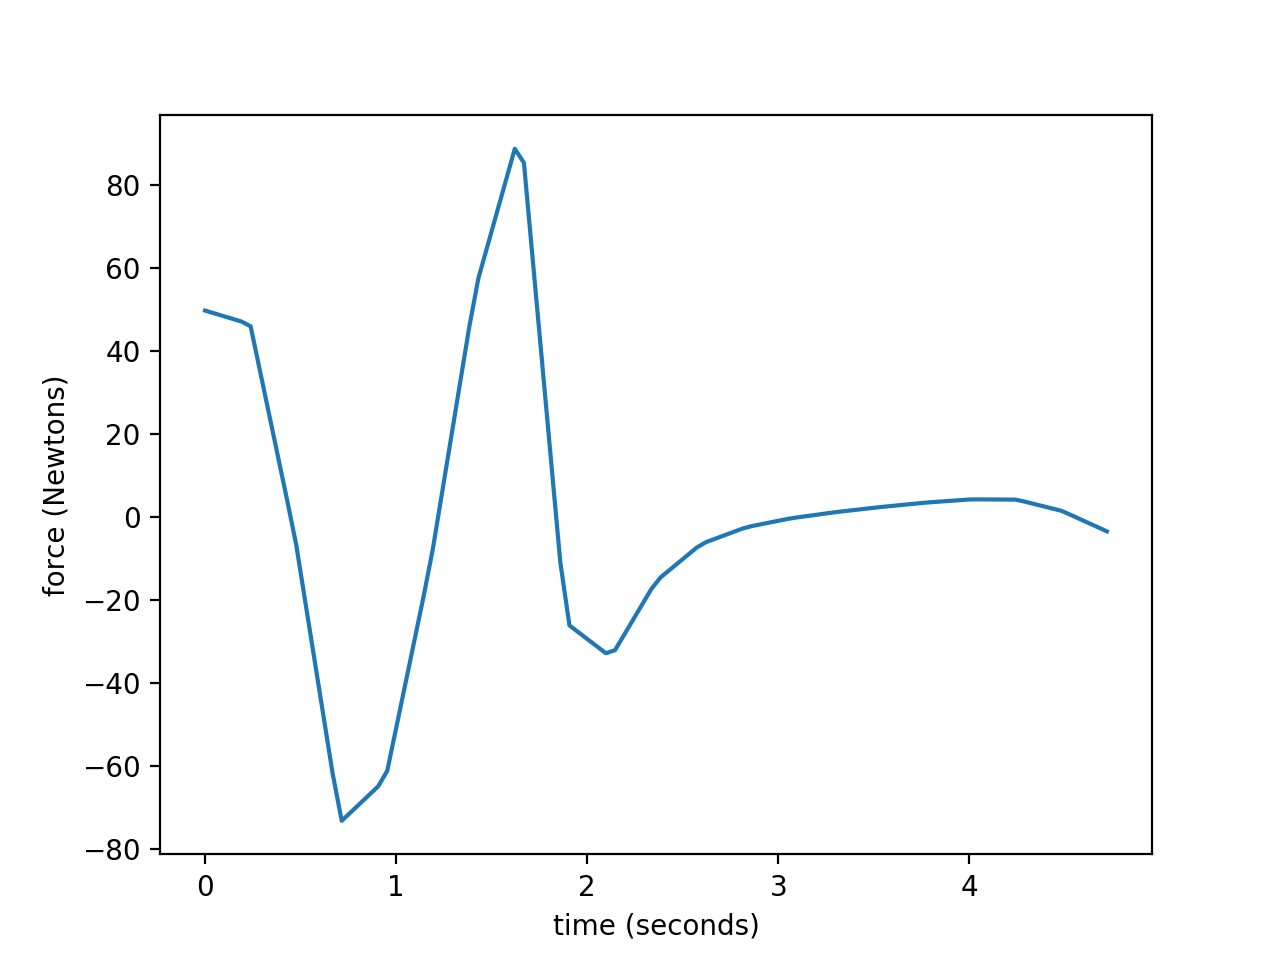
\includegraphics[width=.7\linewidth]{Media/Drake/ExSimple/CartPoleTrajOptDirCol_Solution.png}
\caption{Resulting optimal horizontal force from trajectory optimization of the up-swining and stabilization for the cart-pole.}
\label{fig:cart-pole}
\end{figure}

\subsection{Passive Dynamic Walkers}
Although there currently are no highly-articulated robots found in the Drake examples, it does provide some classic examples of simplified locomotion models. 

\subsubsection{Rimless Wheel}
Simulating the simple dynamics of the rimless wheel model rolling down a declining slope, an continous limit cycle emerges (see Figure \ref{fig:rimlessWheel}).
\begin{figure}[h!]
\centering
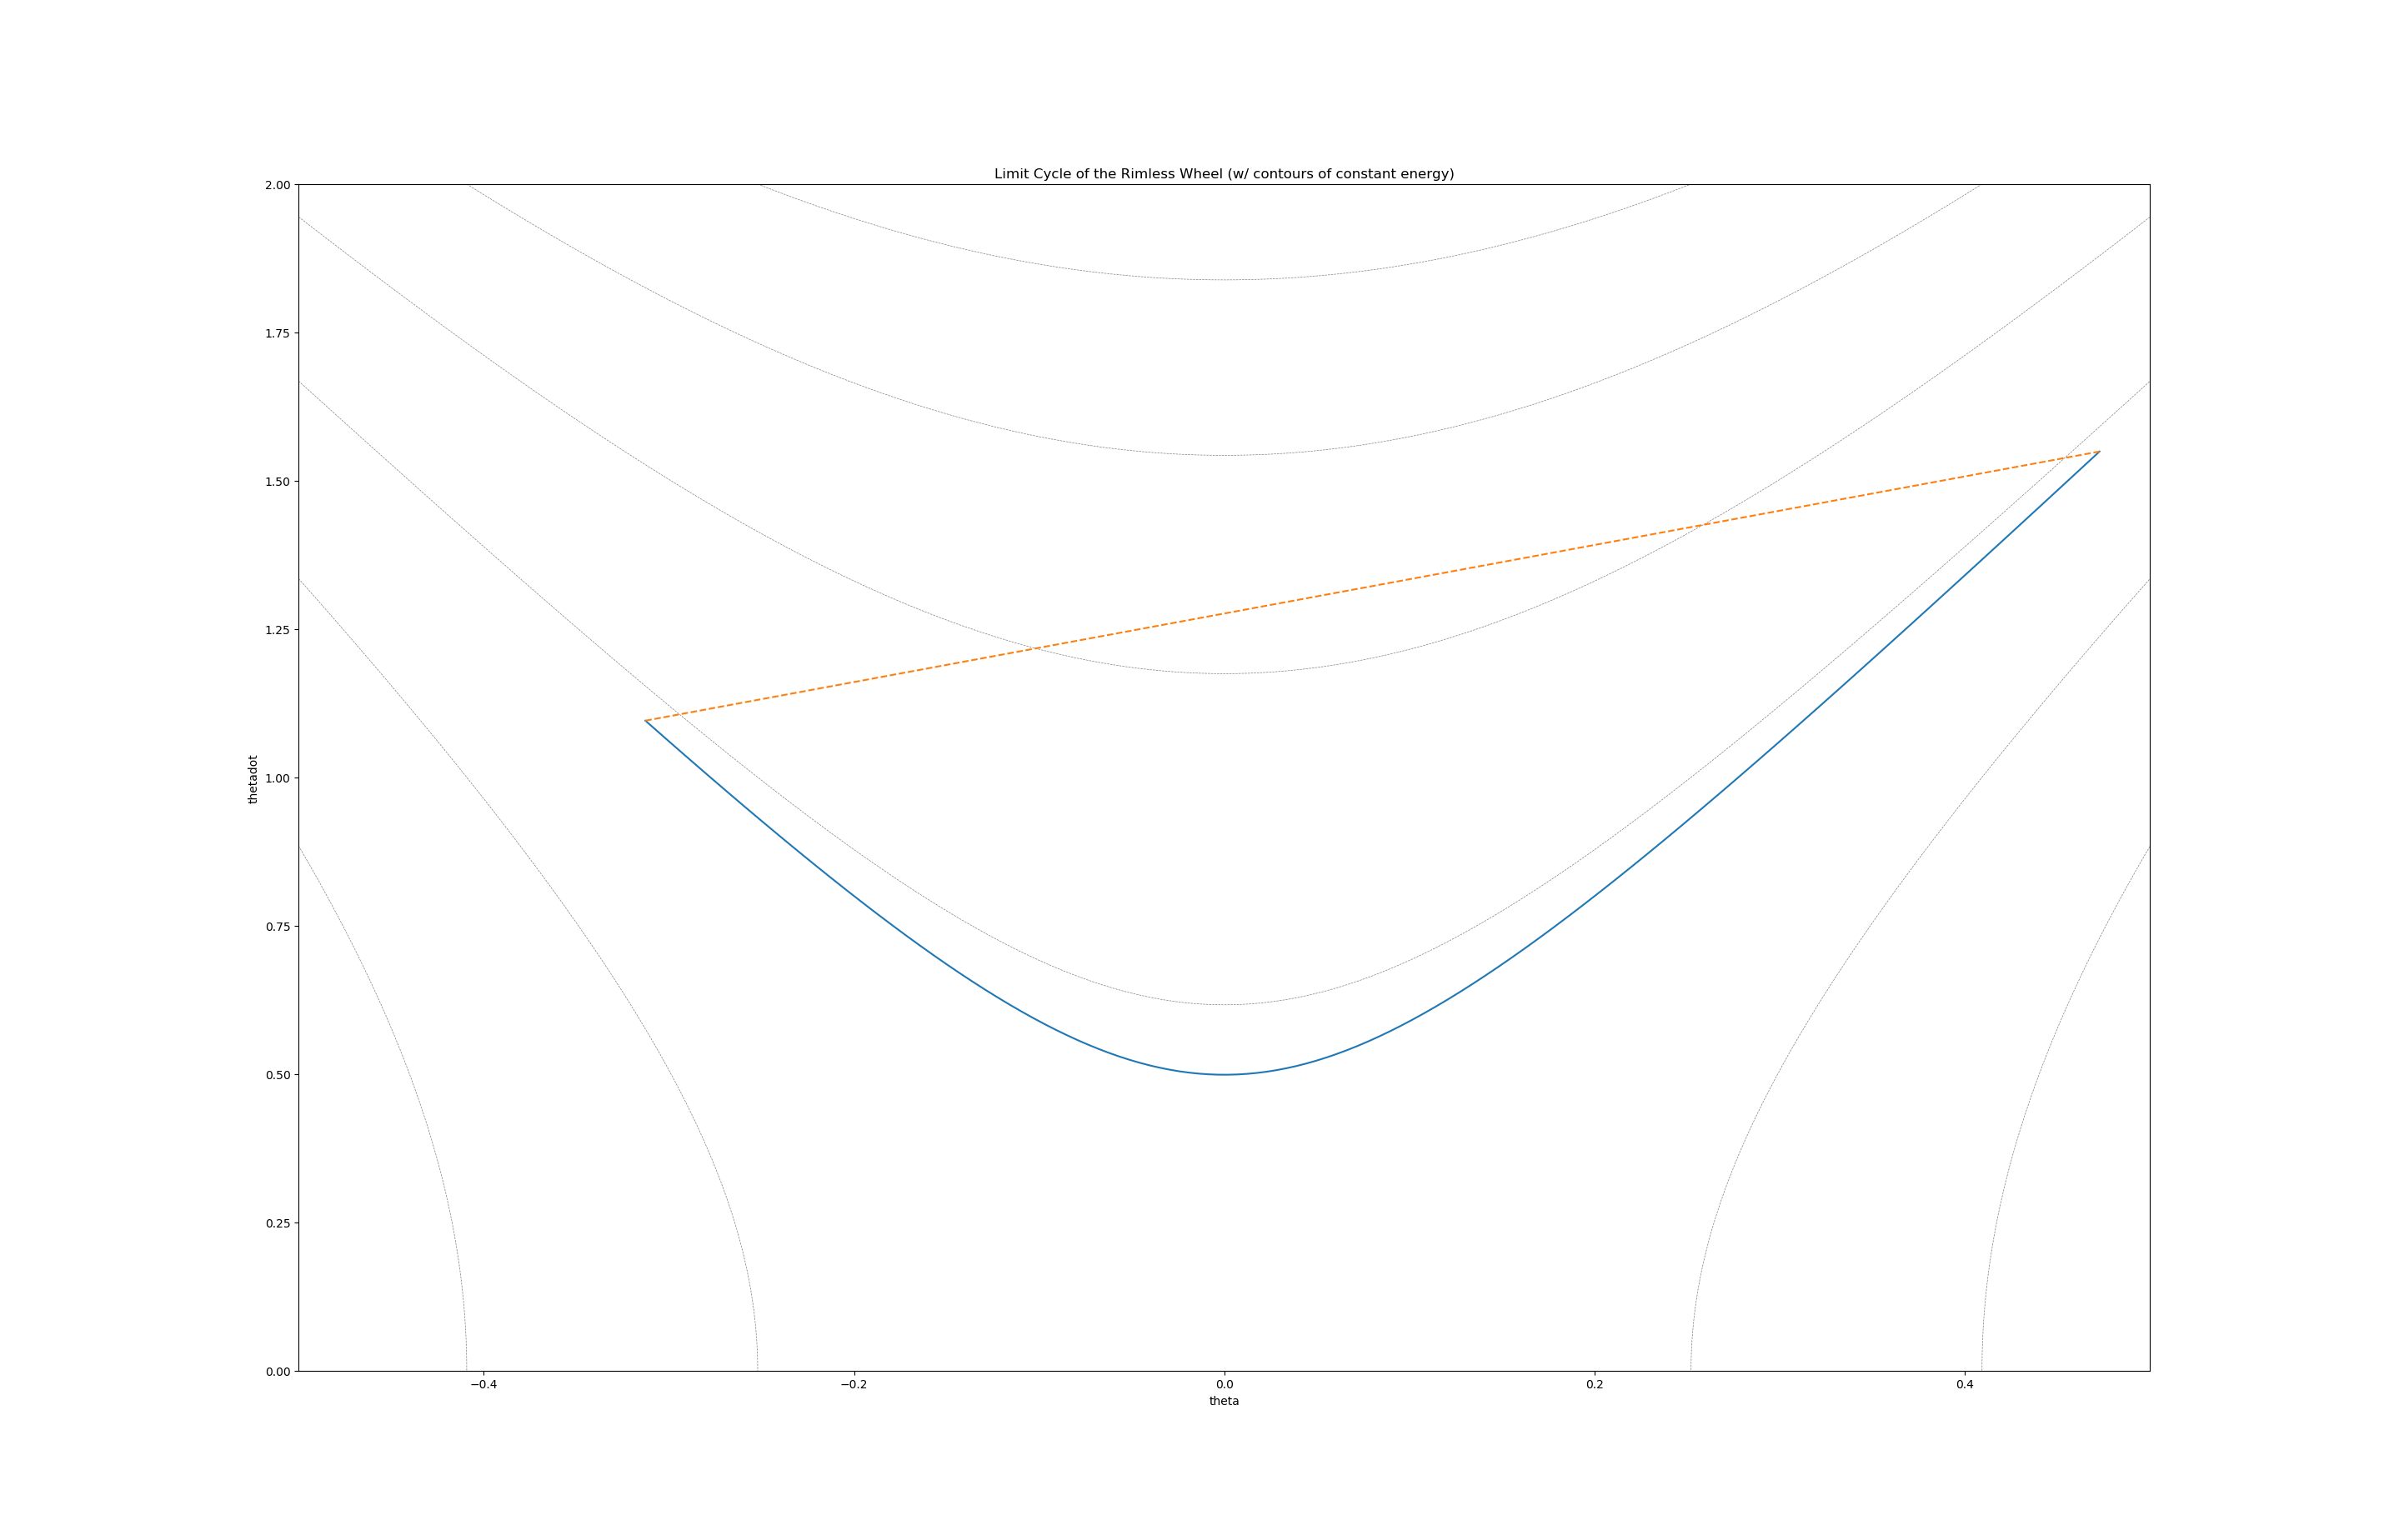
\includegraphics[width=1\linewidth]{Media/Drake/ExSimpleWalking/RimlessWheelDirCol_LimitCycle.png}
\caption{Results for an energy-optimal limit cycle for the rimless wheel using direct collocation trajectory optimization.}
\label{fig:rimlessWheel}
\end{figure}

\subsubsection{Compass Gait}
The compass gait is a simple bipedal walking model containing two links and three pointmasses. For further details on the system visit \url{http://underactuated.csail.mit.edu/simple_legs.html#section2}. 

Simulating the system dynamics for a declining slope results in periodic motions (see Figure \ref{fig:compassGait}).
\begin{figure}[h!]
\centering
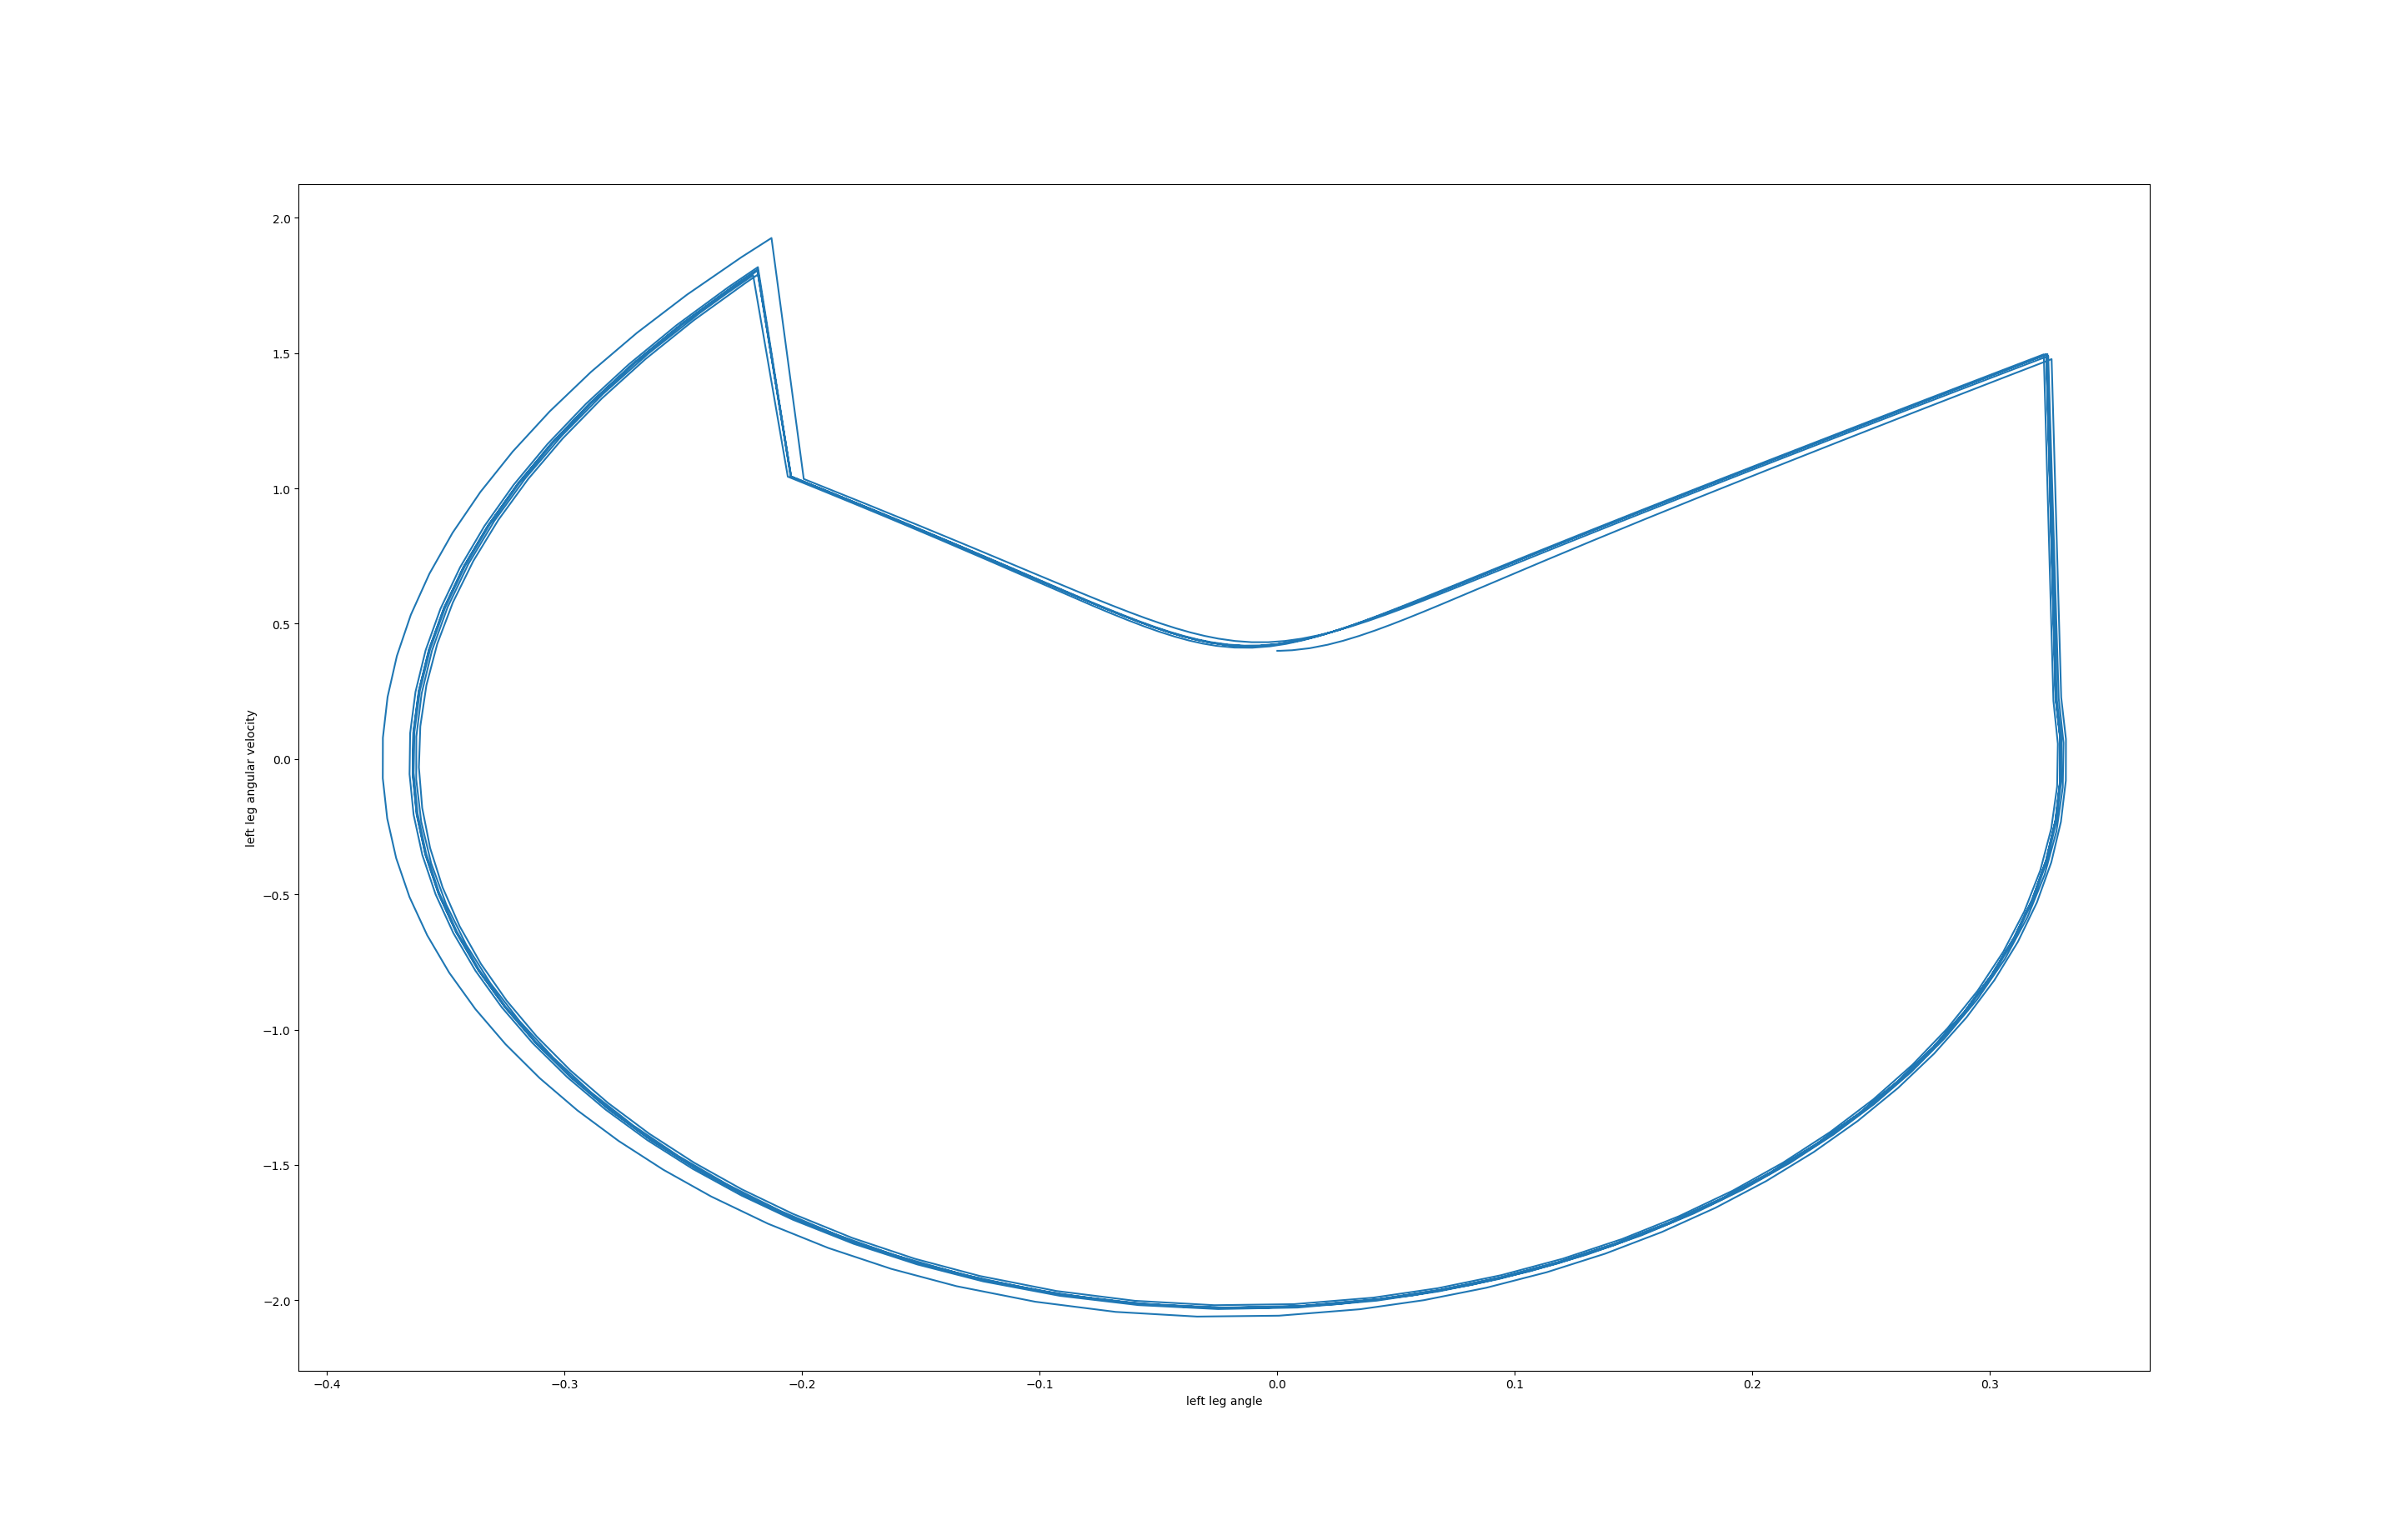
\includegraphics[width=1\linewidth]{Media/Drake/ExSimpleWalking/CompassGait_PhasePlot.png}
\caption{Resulting phase plot of the compass gait reveals periodic orbits.}
\label{fig:compassGait}
\end{figure}


